\documentclass[../../main.tex]{subfiles}
\begin{document}
\section{Validity of a Reissner-Mindlin plate} \label{sec:validity-of-a-plate}

In this section, the validity of a cantilever Reisner-Mindlin plate model is investigated. The idea of the model comes from the beam models in the previous section failing to approximate a cantilever elastic body with a width much larger than it's height. The process of determining the validity of the model follows the same ideas and methodology as in the previous sections, that is established in \cite{LVV09}.

Similarly to how the Timoshenko beam theory improves on the Euler-Bernoulli beam theory by including the shear forces, so does the Reissner-Mindlin plate models improve on classic plate models. The Reissner-Mindlin plate model is a two-dimensional model, and therefore is it of value to investigate the validity of the model using a three-dimensional plate model as a reference.

\subsection{The models}
Form section \ref{ssec:P_Model:ModelProblems}, the cantilever Reissner-Mindlin plate model is given, and is referred to as Problem P-1. The three-dimensional model is the same as used in the previous section, and is referred to as Problem 3D-1 defined in section \ref{ssec:3D_Model:ModelProblems}.

Figure \ref{fig:plate_sbs} shows the two cantilever plates side by side.

\FloatBarrier
\begin{figure}[h!]
	\scalebox{.7}{
		\makebox[\textwidth][c]{
			\caption{Side by side visualization of the cantilever plates.}
			\label{fig:plate_sbs}
			\centering
			\begin{minipage}[b]{0.8\linewidth}
				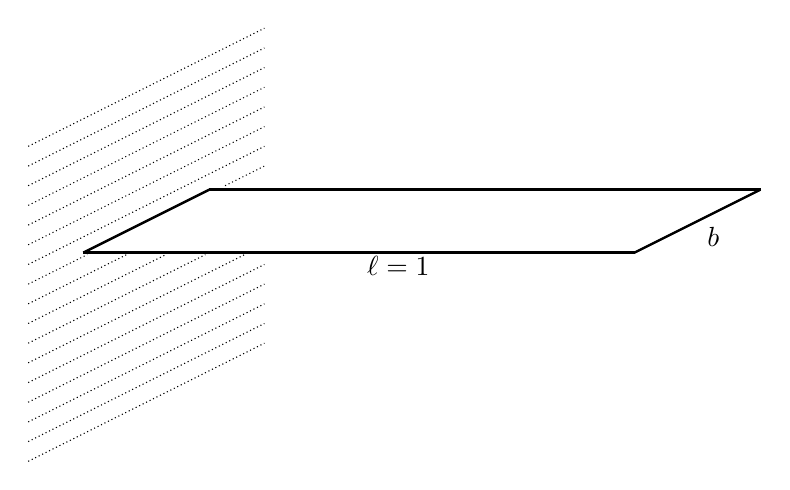
\begin{tikzpicture}
					\draw[line width = 0.3mm] (-0.8,-0.1) -- (6.2,-0.1);
					\draw[line width = 0.3mm] (0.8,0.7) -- (7.8,0.7);
					\draw[line width = 0.3mm] (-0.8,-0.1) -- (0.8,0.7);
					\draw[line width = 0.3mm] (6.2,-0.1) -- (7.8,0.7);
					
					
					
					\draw[scale=0.5, domain=-3:3, smooth, variable=\x,densely dotted] plot ({\x}, {0.5*\x+4});
					\draw[scale=0.5, domain=-3:3, smooth, variable=\x,densely dotted] plot ({\x}, {0.5*\x+3.5});
					\draw[scale=0.5, domain=-3:3, smooth, variable=\x,densely dotted] plot ({\x}, {0.5*\x+3});
					\draw[scale=0.5, domain=-3:3, smooth, variable=\x,densely dotted] plot ({\x}, {0.5*\x+2.5});
					\draw[scale=0.5, domain=-3:3, smooth, variable=\x,densely dotted] plot ({\x}, {0.5*\x+2});
					\draw[scale=0.5, domain=-3:3, smooth, variable=\x,densely dotted] plot ({\x}, {0.5*\x+1.5});
					\draw[scale=0.5, domain=-3:3, smooth, variable=\x,densely dotted] plot ({\x}, {0.5*\x+1});
					
					\draw[scale=0.5, domain=-3:-1.5, smooth, variable=\x,densely dotted] plot ({\x}, {0.5*\x+0.5});
					\draw[scale=0.5, domain=2:3, smooth, variable=\x,densely dotted] plot ({\x}, {0.5*\x+0.5});
					
					\draw[scale=0.5, domain=-3:-0.5, smooth, variable=\x,densely dotted] plot ({\x}, {0.5*\x});
					\draw[scale=0.5, domain=-3:0.5, smooth, variable=\x,densely dotted] plot ({\x}, {0.5*\x-0.5});
					\draw[scale=0.5, domain=-3:1.5, smooth, variable=\x,densely dotted] plot ({\x}, {0.5*\x-1});
					\draw[scale=0.5, domain=-3:2.5, smooth, variable=\x,densely dotted] plot ({\x}, {0.5*\x-1.5});
					\draw[scale=0.5, domain=-3:3, smooth, variable=\x,densely dotted] plot ({\x}, {0.5*\x-2});
					\draw[scale=0.5, domain=-3:3, smooth, variable=\x,densely dotted] plot ({\x}, {0.5*\x-2.5});
					\draw[scale=0.5, domain=-3:3, smooth, variable=\x,densely dotted] plot ({\x}, {0.5*\x-3});
					\draw[scale=0.5, domain=-3:3, smooth, variable=\x,densely dotted] plot ({\x}, {0.5*\x-3.5});
					\draw[scale=0.5, domain=-3:3, smooth, variable=\x,densely dotted] plot ({\x}, {0.5*\x-4});
					
					\node at (7.2,0.1) {$b$};
					\node at (3.2,-0.27) {$\ell = 1$};
										
					
					\draw[line width = 0.2mm] (0.8,0.7) -- (7.8,0.7);
					\draw[line width = 0.2mm] (-0.8,-0.1) -- (0.8,0.7);
					\draw[line width = 0.2mm] (6.2,-0.1) -- (7.8,0.7);
				\end{tikzpicture}
				\subcaption{Reissner-Mindlin cantilever plate}
			\end{minipage}
			\begin{minipage}[b]{0.8\linewidth}
				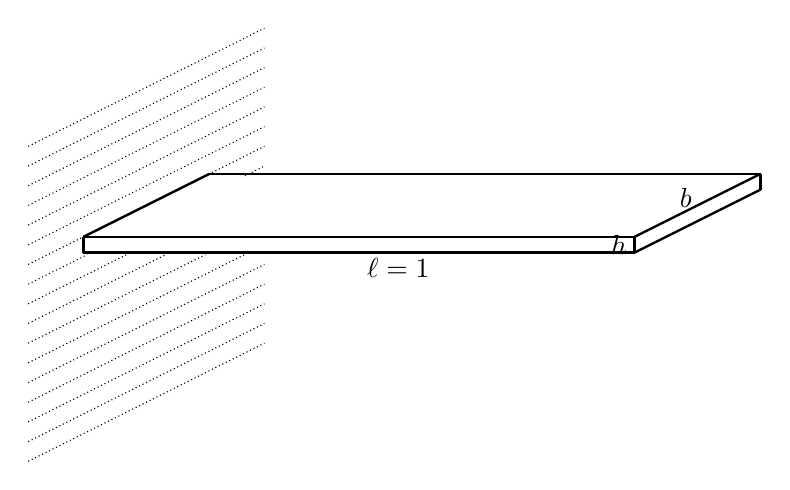
\begin{tikzpicture}
					\draw[line width = 0.3mm] (-0.8,0.1) -- (6.2,0.1);
					\draw[line width = 0.3mm] (-0.8,-0.1) -- (6.2,-0.1);
					\draw[line width = 0.3mm] (6.2,-0.1) -- (6.2,0.1);
					\draw[line width = 0.3mm] (-0.8,-0.1) -- (-0.8,0.1);
					
					\draw[line width = 0.3mm] (0.8,0.9) -- (7.8,0.9);
					\draw[line width = 0.3mm] (7.8,0.7) -- (7.8,0.9);
					
					\draw[line width = 0.3mm] (-0.8,0.1) -- (0.8,0.9);
					\draw[line width = 0.3mm] (6.2,0.1) -- (7.8,0.9);
					\draw[line width = 0.3mm] (6.2,-0.1) -- (7.8,0.7);
					
					
					
					\draw[scale=0.5, domain=-3:3, smooth, variable=\x,densely dotted] plot ({\x}, {0.5*\x+4});
					\draw[scale=0.5, domain=-3:3, smooth, variable=\x,densely dotted] plot ({\x}, {0.5*\x+3.5});
					\draw[scale=0.5, domain=-3:3, smooth, variable=\x,densely dotted] plot ({\x}, {0.5*\x+3});
					\draw[scale=0.5, domain=-3:3, smooth, variable=\x,densely dotted] plot ({\x}, {0.5*\x+2.5});
					\draw[scale=0.5, domain=-3:3, smooth, variable=\x,densely dotted] plot ({\x}, {0.5*\x+2});
					\draw[scale=0.5, domain=-3:3, smooth, variable=\x,densely dotted] plot ({\x}, {0.5*\x+1.5});
					\draw[scale=0.5, domain=-3:3, smooth, variable=\x,densely dotted] plot ({\x}, {0.5*\x+1});
					
					\draw[scale=0.5, domain=-3:-1.5, smooth, variable=\x,densely dotted] plot ({\x}, {0.5*\x+0.5});
					\draw[scale=0.5, domain=2.5:3, smooth, variable=\x,densely dotted] plot ({\x}, {0.5*\x+0.5});
					
					\draw[scale=0.5, domain=-3:-0.5, smooth, variable=\x,densely dotted] plot ({\x}, {0.5*\x});
					\draw[scale=0.5, domain=-3:0.5, smooth, variable=\x,densely dotted] plot ({\x}, {0.5*\x-0.5});
					\draw[scale=0.5, domain=-3:1.5, smooth, variable=\x,densely dotted] plot ({\x}, {0.5*\x-1});
					\draw[scale=0.5, domain=-3:2.5, smooth, variable=\x,densely dotted] plot ({\x}, {0.5*\x-1.5});
					\draw[scale=0.5, domain=-3:3, smooth, variable=\x,densely dotted] plot ({\x}, {0.5*\x-2});
					\draw[scale=0.5, domain=-3:3, smooth, variable=\x,densely dotted] plot ({\x}, {0.5*\x-2.5});
					\draw[scale=0.5, domain=-3:3, smooth, variable=\x,densely dotted] plot ({\x}, {0.5*\x-3});
					\draw[scale=0.5, domain=-3:3, smooth, variable=\x,densely dotted] plot ({\x}, {0.5*\x-3.5});
					\draw[scale=0.5, domain=-3:3, smooth, variable=\x,densely dotted] plot ({\x}, {0.5*\x-4});
					
					\node at (6.85,0.6) {$b$};
					\node at (6,0) {$h$};
					\node at (3.2,-0.3) {$\ell = 1$};
					
					% \draw[line width = 0.1mm,->] (9,1) -- (10,1.6);
					% \draw[line width = 0.1mm,->] (9,1) -- (10.4,1);
					% \draw[line width = 0.1mm,->] (9,1) -- (9,-0.1);
					% \node at (9.2,1.4) {$e_3$};
					% \node at (9.7,0.8) {$e_1$};
					% \node at (8.8,0.4) {$e_2$};
				\end{tikzpicture}
				\subcaption{Three-dimensional cantilever plate}
				
			\end{minipage}
		}
	}
\end{figure}
\FloatBarrier

\subsection{Calculating the eigenvalues}
The eigenvalues for both models are calculated using the Finite Element Method. For the plate model, the Finite Element Method is derived in \ref{sec:FEM:Plate} and for the three-dimensional model, the Finite Element Method is derived in \ref{sec:FEM:3D}.

\subsubsection{Problem P-1E}
Find a vector function $u$ and a number $\lambda$ such that
\begin{eqnarray}
	K{u} & = & M\lambda{u}, 
\end{eqnarray} where $K$ and $M$ are the standard Finite Element Method matrices for bi-cubic basis functions. The definition of the matrices are given in \ref{sec:FEM:Plate}.

\subsubsection{Problem 3D-1E}
Find a real number $\lambda$ and a function $\bar{u} \in S^h$ such that
\begin{eqnarray}
	K\bar{u} & = & M\lambda{\bar{u}},
\end{eqnarray} where $K$ and $M$ are the standard Finite Element Method matrices for tri-cubic basis functions. The definition of the matrices are given in section \ref{sec:FEM:3D}.

\subsubsection{Accuracy of the eigenvalues}
Figure \ref{fig:conv_3d_eig} show the rate of convergence of the first 20 eigenvalues of Problem 3D-1E. 

\begin{figure}[H]
    \centering
    \begin{adjustbox}{center}
        \includegraphics[scale=0.7]{Convergence.png}
    \end{adjustbox}
    \caption{Rate of convergence of the first 20 eigenvalues.}
    \label{fig:conv_3d_eig}
\end{figure}
\textcolor{red}{Update this figure.}

The number of elements can be chosen so that at least the first 10 eigenvalues are accurate to 5 significant digits.

\subsection{Comparing the mode shapes}
\subsection{Comparing the mode shapes}
\FloatBarrier
\begin{figure}[h!]
	\scalebox{.8}{
		\makebox[\textwidth][c]{
			\centering
			\begin{minipage}[b]{0.8\linewidth}
				\includegraphics[width=1\linewidth]{Plate2.png}
				\subcaption{Plate - $\lambda_5 = 0.643$}
				\label{fig:minipage2}
			\end{minipage}
			\begin{minipage}[b]{0.8\linewidth}
				\includegraphics[width=1\linewidth]{3D2.png}
				\subcaption{3D Model - $\lambda_5 = 0.645$}
				\label{fig:minipage1}
			\end{minipage}
	}}
	\scalebox{.8}{
		\makebox[\textwidth][c]{
			\centering
			\begin{minipage}{.8\textwidth}
				\centering
				\includegraphics[width=1\linewidth]{Plate1.png}
				\subcaption{Plate - $\lambda_6 = 1.92$}
				\label{fig:minipage1}
			\end{minipage}
			\begin{minipage}{.8\textwidth}
				\centering
				\includegraphics[width=1\linewidth]{3D1.png}
				\subcaption{3D Model - $\lambda_7 = 1.92$}
				\label{fig:minipage2}
			\end{minipage}
	}}
	\scalebox{.8}{
		\makebox[\textwidth][c]{
			\centering
			\begin{minipage}[b]{0.8\linewidth}
				\includegraphics[width=1\linewidth]{Plate3.png}
				\subcaption{Plate - $\lambda_8 = 2.74$}
				\label{fig:minipage1}
			\end{minipage}
			\quad
			\begin{minipage}[b]{0.8\linewidth}
				\includegraphics[width=1\linewidth]{3D3.png}
				\subcaption{3D Model - $\lambda_8 = 2.74$}
				\label{fig:minipage2}
			\end{minipage}
	}}
	\scalebox{.8}{
		\makebox[\textwidth][c]{
			\centering
			\begin{minipage}[b]{0.8\linewidth}
				\includegraphics[width=1\linewidth]{Plate4.png}
				\subcaption{Plate - $\lambda_{12} = 8.96$ (Side view)}
				\label{fig:minipage2}
			\end{minipage}
			\quad
			\begin{minipage}[b]{0.8\linewidth}
				\includegraphics[width=1\linewidth]{3D4.png}
				\subcaption{3D Model - $\lambda_{14} = 9.01$ (Side view)}
				\label{fig:minipage2}
			\end{minipage}
			\caption{Comparison of Mode Shapes of the 3D model and the plate model. $b = 1/20$, $d = 1$.}
	}}
\end{figure}

\FloatBarrier


Let $b= 1$ and $\alpha= 4800$ so that $h= \frac{1}{2}$.\\

\begin{figure}[h!]
	\scalebox{.8}{
		\makebox[\textwidth][c]{
			\centering
			\begin{minipage}{.8\textwidth}
				\centering
				\includegraphics[width=1\linewidth]{3Dnp1.png}
				\subcaption{3D Model - $\lambda_{6} = 1.35$ (Top view)}
				\label{fig:minipage1}
			\end{minipage}
			\begin{minipage}{.8\textwidth}
				\centering
				\includegraphics[width=1\linewidth]{3Dnp2.png}
				\subcaption{3D Model - $\lambda_{13} = 7.80$ (Top view)}
				\label{fig:minipage2}
			\end{minipage}
	}}
	\caption{Examples of non-plate mode shapes.}
\end{figure}


\subsection{Comparing the eigenvalues}


\end{document}